% Partie 1.1 - l'IoT %

\subsection{L'IoT}

\textit{L'Internet of Things}, que nous appellerons maintenant IoT pour le reste de ce rapport, se traduit littéralement comme l'Internet des Objets, mais qu'est-ce-qu'un objet? Dans le monde de l'IoT les objets peuvent se référer à des biens (comme des meubles ou de l'électroménager), des machines, des véhicules, des immeubles ou bien même à quelque chose d'organique comme un être vivant (Homme ou animal), une plante, des sols (pour les cultures).

Alors la question est : Comment pouvons nous tous connecter ? En effet, comment faire en sorte qu'une plante possède un accès réseau. C'est cela que l'IoT veut définir et représente, une connectivité pour tout.

Mais d'abord que veut dire le mot connecter ? Prenons l'exemple d'une chaise, le fait qu'elle soit connectée veut dire que je peux avoir accès à de l'information la concernant, depuis n'importe où, grâce à un accès à Internet, par exemple, est-elle occupée? Si oui, qui est assis dessus? Pour cela nous avons besoin de donner certains attributs de cette chaise, comme un numéro d'identification unique, une manière de la distinguée d'un autre objet. 

Grâce à \textbf{IPv6}, nous pouvons maintenant affecter une adresse unique à tout sans limite réel car l'espace adressable est sans limite pratique (mais il y a bien sur une limite physique). IPv4 est déjà dépassée en terme de capacité d'adressage depuis longtemps mais grâce à des mécanismes comme le NAT/PAT, IPv4 est encore utilisé. Nous reviendrons sur IPv6 un peu plus tard dans ce rapport lors de notre présentation de 6LoWPAN.

Ensuite, nous avons besoins de donner à la chaise un moyen de communiquer avec le monde, soit de manière filaire ou sans fil grâce à des antennes. D'où la nécessiter des protocoles réseaux qui vont devoir transporter les informations, malheureusement ceux que nous utilisons dans la vie tous les jours ne sont pas vraiment adaptées (IPv4, IPv6, Wi-Fi, ...) à l'IoT, de part leur consommation électrique ou de bande-passante. C'est pourquoi de nouveaux protocoles ont vu le jour, spécialement adaptés à ces besoins. Certain se concentre sur la puissance d'émission et d'autre sur la fiabilité dans les milieux bruités, mais tous prennent en compte certaines contraintes de l'IoT.

Aussi, nous parlons d'information et de données mais il faut bien les générer, pour cela nous utilisons différents types de capteurs, comme par example de pression pour savoir si notre chaise est occupé. Un autre type de capteur pourrait être une puce de localisation, ou bien même un capteur d'identification qui pourra nous dire qui est assis sur notre chaise et qui l'a été. De nos jours les capteurs sont extrêmement petits mais ont quand même certaines capacités comme de la mémoire, ce qui est très pratique en cas de coupure temporaire du réseaux, en effet, les données ne sont pas forcément perdue.

\begin{figure}[H]
\begin{center}
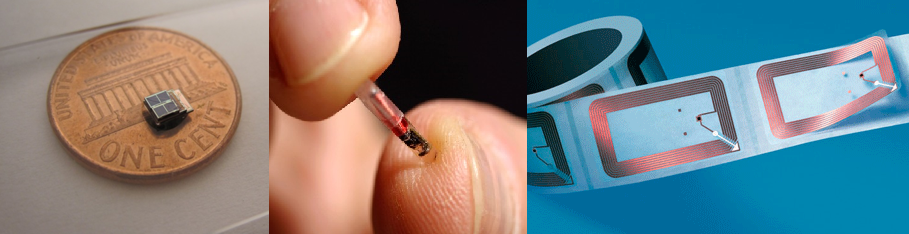
\includegraphics[width=15cm]{\rpDossier/images/capteurs.png}
\end{center}
\caption{Exemple de capteurs}
\label{conflinphone}
\end{figure}

Quelles seront les impacts et les possibilités de l'IoT ? Nous ne sommes limités seulement par notre imagination car nous changeons l'approche de voir et de connecter les objets.

Prenons quelques exemples pour montrer l'intérêt de l'IoT. Le \textit{monitoring} ne se résume pas qu'aux réseaux et machines, on peut aussi l'appliquer pour surveiller l'état d'un patient en médecine. Imaginons quelqu'un avec un problème cardiaque, il possède un pacemaker qui est "connecté", cela veut dire qu'une application sur son téléphone peut dire à cette personne l'état de son cœur, mais aussi à son hôpital. Dans le cas d'un défaillance, une alerte est lancée à l'hôpital qui peut envoyer immédiatement une ambulance, quand à la localisation ils peuvent utiliser un tracker GPS intégré au tout.

Grâce à des algorithmes puissant, on pourra même prédire un potentiel problème sans que le patient vienne faire des visites de contrôles régulières, son pacemaker enverra les données pour lui. Avec le nombre de personne de plus de 65 qui va doubler dans peu de temps, la e-santé et la télé-médecine vont devenir un des plus gros secteurs de l'IoT. 

Les tracas de quotidiens comme la perte de ses clefs ne seront plus un problème, en effet, dans le monde de l'IoT vos clés sont géo-localisables. Cela peut s'appliquer à plein de choses, si ce n'est à toutes, vous ne perdrez plus jamais rien.

Si nous savons où les choses sont et dans quelles états elles sont, nous pouvons mieux les manager. Prenons le cas du trafic en ville, si je sais où les voitures sont et ou elles vont, nous pouvons potentiellement éliminer les bouchons, optimiser les trajets et rediriger les flux plus facilement. Il en va de même pour l'énergie, si nous savons où l'énergie est requise, nous pouvons adapter la production et optimiser les coûts.

L'IoT permet aussi de déléguer du contrôle, toujours dans une optique d'optimisation énergétique, nous pouvons déléguer l'heure de départ d'une machine à laver, d'un lave-vaisselles à un contrôleur distant qui lancera le programme au moment où l'énergie sera la moins chère.

% Video-games

Un autre marché que l'IoT va investir est le jeux-vidéo.


% Privacy %

% Security %